\documentclass[12pt,epsf,makeidx,oneside]{book}

%\input{vhdllisting.tex}

\usepackage[a4paper, total={6.5in, 10in}]{geometry}
\usepackage{subfigure}
\usepackage{epsfig}
\usepackage{graphicx}
\usepackage{listings}
\usepackage{xcolor}
\usepackage{color}

\usepackage{url}
\usepackage{graphicx}
\usepackage{listings}
\usepackage{hyperref}
\usepackage[absolute,overlay]{textpos}
\usepackage{wasysym}
\usepackage[font=small,labelfont=bf]{caption}
\usepackage{adjustbox}
\usepackage{multirow}
\usepackage{enumitem}

\graphicspath{{./}{./img/}}  

\begin{document}

\lstset{backgroundcolor=\color{lightgray}}

\setcounter{tocdepth}{3}
\setcounter{secnumdepth}{3}

\begin{titlepage}
  \begin{center}
    \vspace*{4cm}
    \Huge{\bf Lab Workbook}\\
    \Large{SS 2024}\\
    \vspace{1.5cm}
    \Huge{Industrial Hardware Verification}\\
    \vspace{3cm}
    \Large{
      Jakob Lechner \\
      Markus Ferringer \\
    }
    \vspace*{3cm}
    \Huge{
      Part 3: PSL
    }
  \end{center}
\end{titlepage}

\tableofcontents

\chapter*{Lab Mode}
\begin{itemize}[noitemsep]
  \item You have to elaborate these exercises on your own. This lab part is {\bf not} a team effort.
  \item We provide stubs containing basic templates for you which are to be extended with your implementations
  \item Questions are to be ansered in the respective source-files of the corresponding exercise. Just add appropriate comments at the end
  \item I strongly recommend to read through an entire task before starting with the implementation (including the questions section). You will sometimes find hints later that might simplify things
  \item Once done with all exercises, please execute {\tt ./make.sh clean} in each folder, zip {\bf everything} (including makefiles, scripts, and frameworks) and submit it via TUWEL
\end{itemize}

\chapter*{Remarks}
The syntax presented in the lextures was mostly based on Verilog flavor (because it's shorter and thus better fits on slides). Keep this in mind esp. for locial operators like !, \&\&, $||$: Those have to be replaces by {\tt not, and, or}. Most of the time,
the equality operator (or assignment operator) {\tt =} is to be replaced with {\tt is}.
I found that esp. LTL style is not supported according to the standard. For example, I could not get the {\tt next} command running in combination with specifying a range, like {\tt next[2 to 3]} or {\tt next[2:3]}.

Just try different combinations / styles, and be sure not to leave out any braces. PSL is VERY picky about braces. 

%%%%%%%%%%%%%%%%%%%%%%%%%%%%%%%%%%%%%%%%%%%%%%%%%%%%%%%%%%%%%%%%%%%%%%%
%%% VHDL                                                            %%%
%%%%%%%%%%%%%%%%%%%%%%%%%%%%%%%%%%%%%%%%%%%%%%%%%%%%%%%%%%%%%%%%%%%%%%%
\chapter{PSL}

%%%%%%%%%%%%%%%%%%%%%%%%%%%%%%%%%%%%%%%%%%%%%%%%%%%%%%%%%%%%%%%%%%%%%%%
\section{Exercise 1: PSL from Waveform}
\begin{itemize}
  \item For the given waveforms, write PSL assertions that check the waveforms as depicted.
  \item In this exercise, the signals do not depend on each other, so you just have to describe the depicted, static waveform in PSL
\end{itemize}
% Wavedrom
% { signal: [
%   { name: "clk",  wave: 'p.....' },
%   { name: "a",    wave: '01.010' },
%   { name: "b",    wave: '0.10.1' },
%   { name: "c",    wave: '01.01.' },
% ],
%  head:{
%    tock:0,
%    every:1
%  }
% }
\begin{center}
  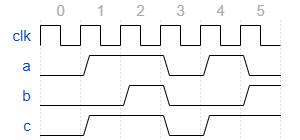
\includegraphics[width=0.4\textwidth]{ex1}
\end{center}

\subsection{Task 1 [1 Point]}
  \begin{itemize}
    \item Describe the given trace using assertions in LTL style
  \end{itemize}
 
\subsection{Task 2 [1 Point]}
  \begin{itemize}
    \item Describe the given trace using assertions in SERE style
  \end{itemize}


%%%%%%%%%%%%%%%%%%%%%%%%%%%%%%%%%%%%%%%%%%%%%%%%%%%%%%%%%%%%%%%%%%%%%%%
% Wavedrom
%{ signal: [
%  { name: "clk1",  wave: '01010101010' },
%  { name: "pi",    wave: '0..1.0.....' },
%  { name: "clk2",  wave: 'p..........' },
%  { name: "po",    wave: '0.......10.' },
%  
%  ],
% head:{
%   tock:0,
%   every:1
% }
%}
\section{Exercise 2: Pulse Clock Crosser}
\begin{center}
  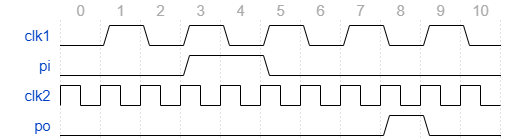
\includegraphics[width=0.6\textwidth]{ex2}
\end{center}
The unit under test is a Pulse Clock Crosser. As you can see in the waveform, it crosses a single-cycle pulse
from clock domain 1 to a single-cycle pulse in clock domain 2. Those clock domains can be totally unrelated.

\subsection{Task 1 [2 Points]}
Write PSL expressions, either LTL or SERE style (or both), to cover the following requirements:
\begin{itemize}
  \item The input {\tt pi} is high for exactly one cycle at a time. It belongs to clock {\tt clk1}
  \item The output {\tt po} is high for exactly one cycle at a time. It belongs to clock {\tt clk2}
  \item After input {\tt pi} has been asserted, it must not be asserted again before the corresponding {\tt po} has been asserted first
  \item After input {\tt pi} has been asserted, the output {\tt po} must be asserted eventually
  \item After input {\tt pi} has been asserted (at {\tt clk1}), the output {\tt po} must not be asserted for at least 2 clock cylces (of {\tt clk2}). There are internal clock crossers, and they need some time. Notice: This does not mean that {\tt po} must be asserted in the 3rd cycle - it could take longer!
\end{itemize}


%%%%%%%%%%%%%%%%%%%%%%%%%%%%%%%%%%%%%%%%%%%%%%%%%%%%%%%%%%%%%%%%%%%%%%%
\section{Exercise 3: Check Waveform}

\subsection{Task 1 [1 Point]}
\begin{center}
  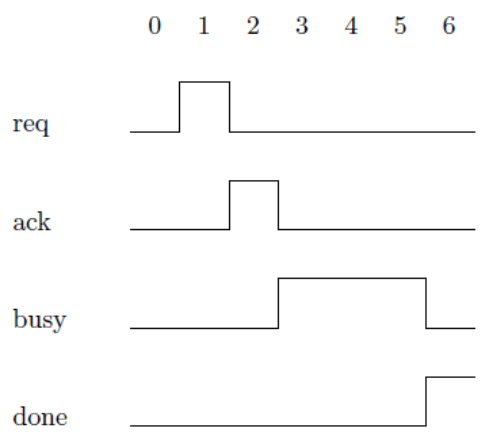
\includegraphics[width=0.3\textwidth]{ex3_1a} \vspace*{0.5cm}
  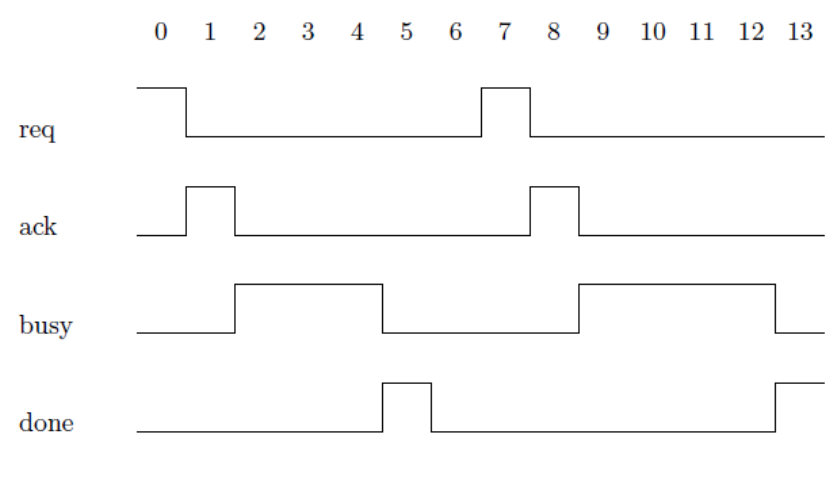
\includegraphics[width=0.4\textwidth]{ex3_1b} \\
  (a) \hspace*{5cm}(b)
\end{center}
There are waveforms (a) and (b) and PSL expressions p1, p2, p3. Check if the PSL expressions hold for the given waveforms. If not, state in which cycle they fail, and why.
\begin{lstlisting}[gobble=2,language=vhdl]
  p1: assert always {req} |=> {ack;busy;busy;busy;done};
  p2: assert always {req} |=> {ack ; busy[*3] ; done}; 
  p3: assert always {req} |=> {ack ; busy[*3:5] ; done};
\end{lstlisting}

\subsection{Task 2 [1 Point]}
\begin{center}
  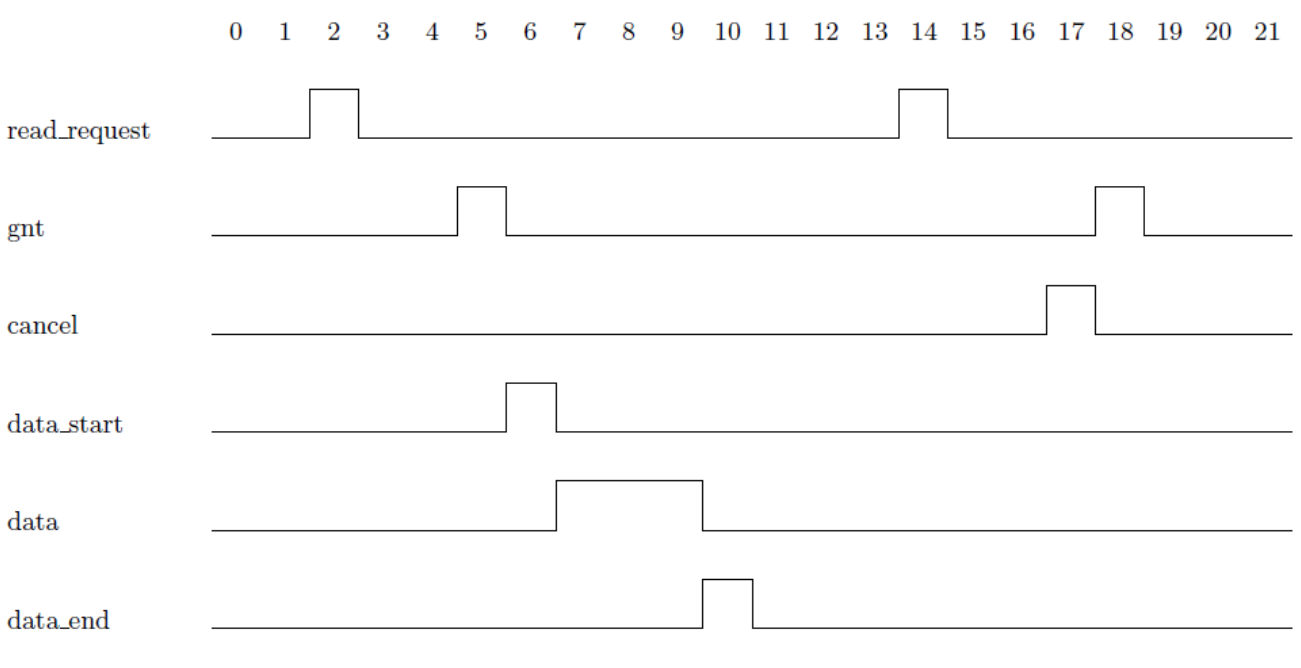
\includegraphics[width=0.8\textwidth]{ex3_2} \\
  (a)
\end{center}
There is waveform (a) and PSL expressions p1, p2. Check if the PSL expressions hold for the given waveform. If not, state in which cycle they fail, and why.
\begin{lstlisting}[gobble=2,language=vhdl]
  p1: assert always
    {{read_req ; [*0:4] ; gnt} && {cancel[=0]}} |=>
    {data_start ; data[*] ; data_end};
  p2: assert always
    {{read_req ; [*0:4] ; gnt} & {cancel[=0]}} |=>
    {data_start ; data[*] ; data_end};
\end{lstlisting}



%%%%%%%%%%%%%%%%%%%%%%%%%%%%%%%%%%%%%%%%%%%%%%%%%%%%%%%%%%%%%%%%%%%%%%%
% Wavedrom
% { signal: [
%   { name: "clk",      wave: 'p...................' },
%   { name: "rd_ena",   wave: '01.....0.1....0.1.0.', node: '.a.....b.c....d.f.g' },
%   { name: "rd_done",  wave: '0......10.....10..10', node: '.......h......i...j' },
%   { name: "rd_valid", wave: '0.1..010..10.10..10.', node: '..k.......m......n' },
%   { name: "rd_burst", wave: 'x4.....x.4....x.4.x.', data: [ '4', '2', '1'] },
%   { name: "rd_data",  wave: 'x.555x5x..5x.5x..5x.' },
%   
%   ],
%   edge: [
%     'a~>k', 'c~>m', 'f~>n', 'b~>h', 'd~>i', 'g~>j'
%   ],
%  head:{
%    tock:0,
%    every:1
%  }
% }
\pagebreak
\section{Exercise 4: Burst Reads}
\begin{center}
  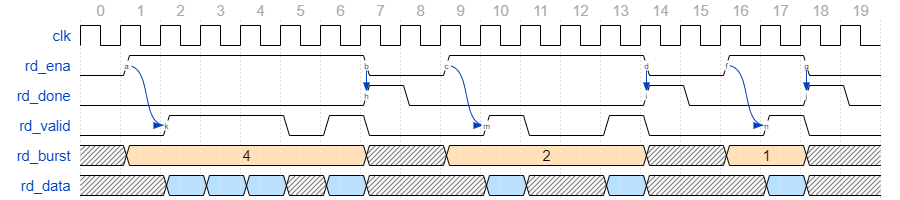
\includegraphics[width=0.9\textwidth]{ex4}
\end{center}
The image shows a typical waveform of a burst-read interface:
\begin{itemize}
  \item With {\tt rd\_ena}, also {\tt rd\_burst} is asserted.
  \item {\tt rd\_burst} is in range 1-7 and defines the number of data values to be read
  \item Starting with the next cycle, data is applied by asserting {\tt rd\_valid} (and setting {\tt rd\_data})
  \item After the last transmitted word, {\tt rd\_done} is asserted
  \item {\tt rd\_valid} is not necessarily high for the entire burst. Pauses are allowed
  \item However, the first data value directly after {\tt rd\_ena} is asserted, is always valid
  \item {\tt rd\_ena} and {\tt rd\_done} are never active at the same time
\end{itemize}

\subsection{Task 1 [4 Points]}
For the above waveform with the given specification, define the following PSL statements. Please take a note at the hints for this exercise.
\begin{itemize}
  \item Check that whenever {\tt rd\_ena} becomes 1 (i.e., changes from 0 to 1), the next cycle always contains valid data (with {\tt rd\_ena} still asserted and {\tt rd\_done} being deasserted).
  \item Check that when {\tt rd\_ena} becomes 1, it is followed by 1 to 7 assertions of {\tt rd\_valid} (with {\tt rd\_done}=0), followed by a single assertion of {\tt rd\_done}. Notice that {\tt rd\_valid} can have interruptions.
  \item Check that {\tt rd\_ena} stays asserted until {\tt rd\_done} is asserted
  \item Check that when {\tt rd\_done} is asserted, the correct number of {\tt rd\_valid} cycles (according to {\tt rd\_burst}) have occured
\end{itemize}

{\bf Hints: } There are probably various ways how the above requirements can be checked. I will provide hints for one possible solution:
\begin{itemize}
  \item In the PSL file, you can define VHDL signals. Define {\tt burst} of type {\tt integer}. You can just write ``inline VHDL'' like every other PSL expression.
  \item Make a concurrent (VHDL-)assignment to {\tt burst} such that it assigns the current value of {\tt rd\_burst} at the rising edge of {\tt rd\_ena}, and that it decrements itself when both {\tt rd\_ena} and {\tt rd\_valid} are asserted (otherwise, leave unaffected).
  \item You can then use the signal {\tt burst} inside a PSL expression and check if it is indeed 0 when {\tt rd\_done} is asserted
  \item You can use {\tt rising\_edge()} inside PSL expressions
\end{itemize}


\end{document}
